\section{MODULO: PROCESAMIENTO DE IMÁGENES}

\subsection{Red neuronal convolucional: SqueezeDet}

\subsubsection{Introducción}

A lo largo de los años se ha logrado ir aumentando la precisión de las redes neuronales convolucionales con distintos tipos de arquitecturas a tal punto en el que hoy en día se pueden encontrar distintas arquitecturas que cumplan un nivel de precisión que se necesite.\par
Dado cierto nivel de precisión es muy útil tener una arquitectura de CNN (convolutional neural network) con menos parámetros, en especial cuando a un proyecto embebido se refiere.\par
\bigbreak
Algunas ventajas de utilizar redes mas pequeñas son: 
\begin{itemize}
    \item Los FPGA suele tener menos de 10 MBytes de memoria en el chip y no suelen tener memoria o almacenamiento fuera del chip. Un modelo suficientemente pequeño podría almacenarse directamente en la FPGA, mientras que los fotograma de vídeo se transmiten en tiempo real a través de ella. 
    \item Cuando se habla de entrenamiento distribuido, la carga de trabajo para entrenar el modelo se divide y se comparte entre varios procesadores llamados nodos de trabajo para acelerar y/o paralelizar el entrenamiento. En estos casos tener redes mas pequeñas ayuda a que este tipo de entrenamiento sea aun mas eficiente con la ventaja de que la "performance" de la red no se ve afectada.
    \item Empresas como Tesla copian periódicamente nuevos modelos de sus servidores a los productos de sus clientes (autos), al trabajar con redes mas pequeñas el gasto de exportar estos modelos se vería relativamente disminuido.
\end{itemize}

Una ventaja de esta red en particular es que es susceptible de compresión. En donde combinando grandes técnicas de compresión como "Deep Compression" y la arquitectura de la SqueezeDet se logran reducciones de modelo de hasta 510x veces.
\bigbreak
El objetivo de este modulo es entonces lograr el entrenamiento de una SqueezeDet, con un dataset propio y escribir su implementación en C para poder implementarla en una placa de desarrollo Zybo sobre un SoC Zynq-7000. Con la motivación de estudiar su posible implementación, o acelerado en la FPGA del mismo SoC.

\subsubsection{Arquitectura SqueezeDet}

Tomando como referencia el paper \cite{SQdet} el objetivo general de esta red fue lograr un modelo que tenga muy pocos parámetros y al mismo tiempo mantenga la precisión, para lograr esto lo que se hizo fue a partir de un modelo dado (red neuronal fully connected: SqueezeNet) se la logro comprimir con ciertas perdidas.\par

Tres estrategias se utilizaron para lograr esta compresión: 
\begin{itemize}
    \item \textbf{Estrategia 1:} Remplazar los filtros 3x3 con filtros 1x1. Estos tienen 9 veces menos parámetros.
    \item \textbf{Estrategia 2:} Siendo la cantidad total de parámetros en una CNN con filtros de 3x3 = (números de canales de entrada)(numero de filtros)(3x3) se busca reducir estos, reduciendo los números de canales de entrada, usando capas de compresión que se describen mas adelante.
    \item \textbf{Estrategia 3:} Disminuir la resolución al final de la red para que las capas de convolución tengan mapas de activación grandes. Normalmente la reducción de resolución se diseña en arquitecturas de CNN al establecer el step>1 en algunas de las capas de convolución o agrupación.
\end{itemize}

\paragraph{Macroarquitectura SqueezeDet}\mbox{}\\

La macro-arquitectura se refiere a la organización del nivel de organización del sistema de múltiples módulos dentro de la arquitectura completa de la CNN.\par

En la figura se puede ver la arquitectura de la SqueezeDet. Comienza con una capa de convolución independiente (conv1) seguida de 11 "Fire Modules" y termina con otra capa de convolución independiente. Gradualmente se aumenta el numero de filtros por "Fire Module" desde el principio de la red al final. Además realiza un max-pooling con un stride de 2 despues de las layers conv1, fire3 y fire5. Las ubicaciones de estos pooling hacen referencia a la \textbf{Estrategia 3}.

\begin{center}
    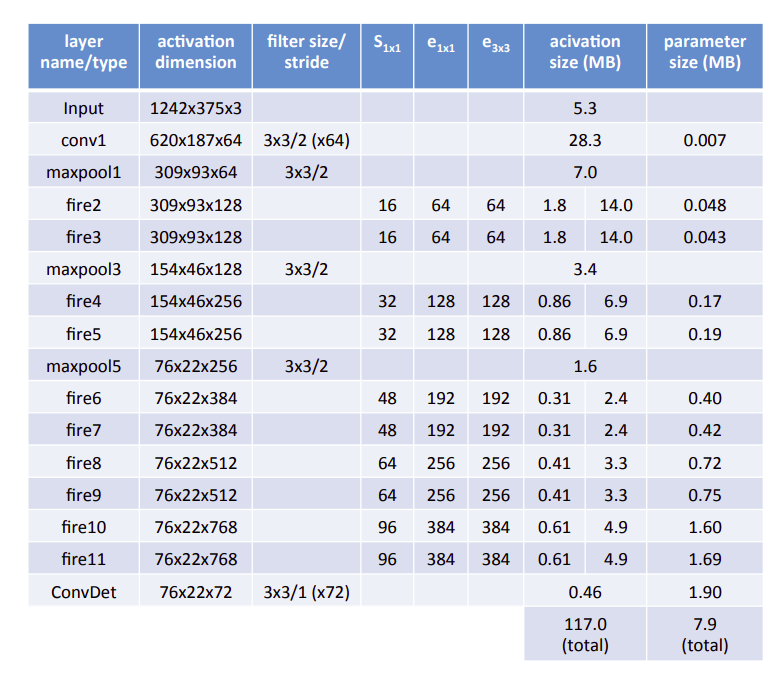
\includegraphics[scale=0.5]{Tesis/Capitulos/03_CAPITULO_1/img/squeezenetmacro.png}
    \captionof{figure}{Arquitectura SqueezeDet}
\end{center}

\paragraph{Microarquitectura SqueezeDet}\mbox{}\\

La micro-arquitectura hace referencia a las capas individuales y los módulos. La operación de convolución ha sido utilizada por al menos 25 años en las CNN. Cuando el desarrollo de las CNN se aplica a imágenes típicamente los filtros de la CNN tienen 3 canales en su primer layer (ej,RGB) y en cada layer siguiente los filtros tienen el mismo numero de canales que el numero de filtros que tuvo la layer anterior. Al diseñar CNN muy profundos, se vuelve tedioso el hecho de estar seleccionando manualmente las dimensiones del filtro, para abordar esto se propuso varios bloques de construcción de nivel superior, o módulos, que luego se combinan para formar una red completa.

\subparagraph{The fire module}\mbox{}\\

Este modulo permite alcanzar las 3 estrategias. Un "Fire Module" se compone de una capa de convolución de compresión (solo tiene filtros de 1x1) que se alimenta a una capa de expansión que tiene una mezcla de filtros de convolución de 1x1 y 3x3 ver figura. El uso de los filtros 1x1 en este modulo es con el propósito de satisfacer la Estrategia 1.

\begin{center}
    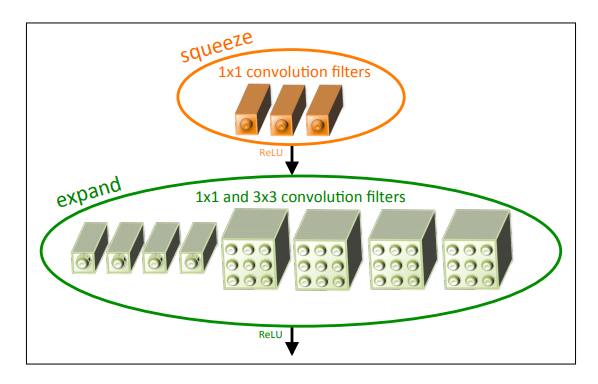
\includegraphics[scale=0.7]{Tesis/Capitulos/02_MARCO_TEORICO/img/firemodule.png}
    \captionof{figure}{The fire module}
\end{center}

Se exponen 3 hiperparámetros dentro del modulo s1x1, e1x1 y e3x3. En donde:

\begin{itemize}
    \item s1x1: Cantidad de filtros en la capa de compresión (todos 1x1).
    \item e1x1: Cantidad de filtros en la capa de expansión (todos 1x1).
    \item e3x3: Cantidad de filtros en la capa de expansión (todos 3x3).
\end{itemize}

Cuando usamos un "Fire Module" configuramos s1x1 para que sea menor que (e1x1 + e3x3) por lo que la capa de compresión ayuda a limitar el numero de canales de entrada a los filtros 3x3 Estrategia 3.

\subsection{Creación de un pequeño dataset propio}

A modo de realizar una primera prueba se llevo a cabo la construcción de un pequeño dataset de 225 imágenes, las cuales fueron etiquetadas con el programa \href{https://alpslabel.wordpress.com/}{\textbf{"Alp’s Labeling Tool (ALT)"}}.

Esta aplicación te permite dibujar rectángulos alrededor de los objetos, nombrar estos rectángulos, rotar la imagen con los rectángulos por completo, guardar toda esta información y volver a cargar más tarde junto con la imagen seleccionada para continuar etiquetando desde donde lo dejaste. Los archivos de etiquetas ".txt" se crean en la misma carpeta que la imagen y contienen etiquetas y sus coordenadas de cuadro delimitador, por lo que una vez completado el trabajo de etiquetado, puede mover los archivos de etiquetas ".txt" relevantes al conjunto de datos real, a las carpetas de "etiquetas" en "tren" y "val".

\begin{center}
    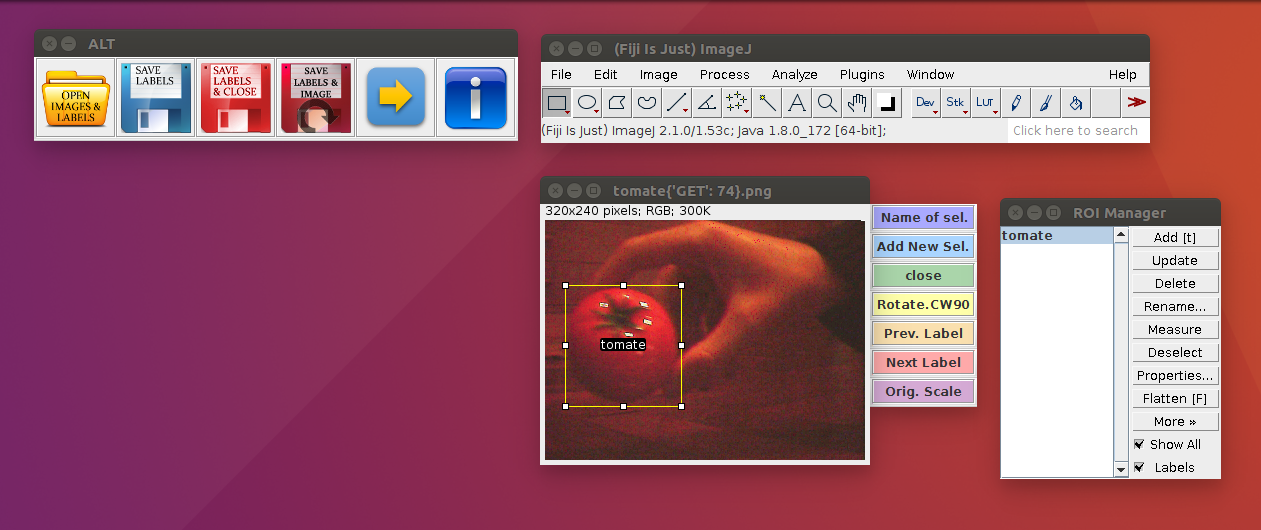
\includegraphics[scale=0.3]{Tesis/Capitulos/03_CAPITULO_1/img/etiquetas.png}
    \captionof{figure}{Pequeño Dataset propio}
\end{center}

\subsection{Entrenamiento de una red SqueezeDet con dataset propio}

Para el entrenamiento de esta red se utilizo un repositorio con la implementación y entrenamiento de la SqueezeDet en Keras (python) el cual se puede encontrar \href{https://github.com/omni-us/squeezedet-keras}{\textbf{"aqui"}}.

Aqui se pueden ver las imágenes utilizadas como validación. El cuadro verde es la etiqueta hecha con Alp’s Labeling Tool y las rojas las predicciones hechas por la red con un threshold en la probabilidad superior al 30\%.

\begin{center}
    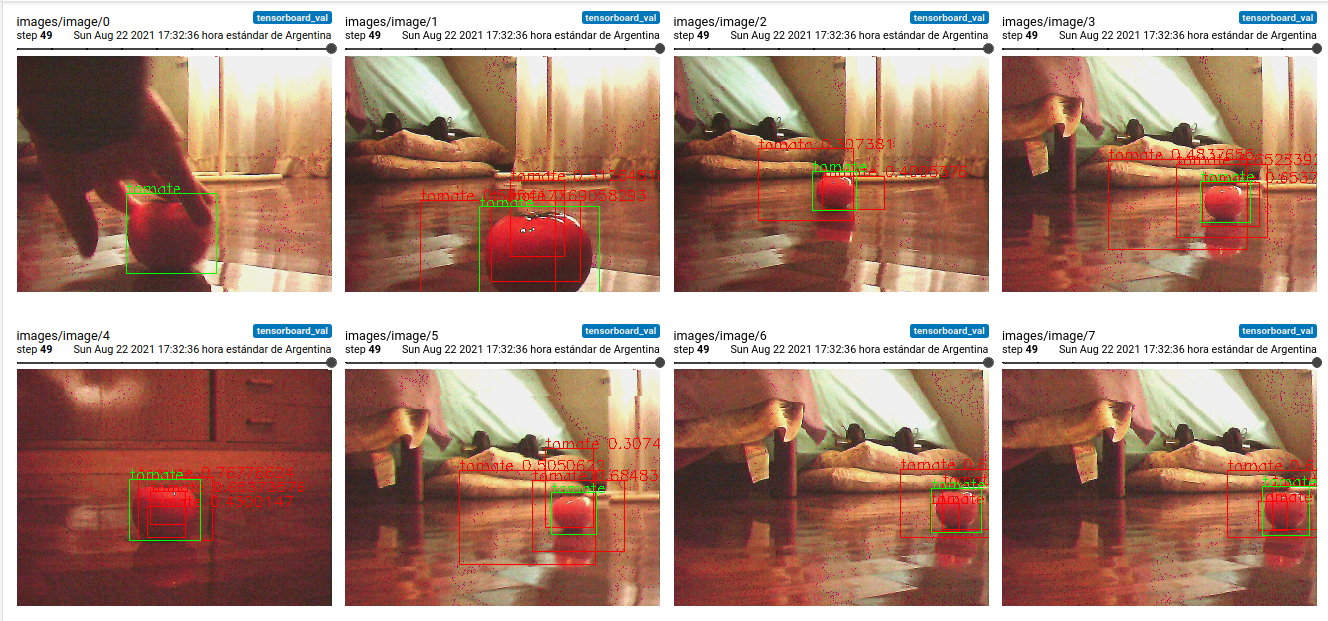
\includegraphics[scale=0.3]{Tesis/Capitulos/03_CAPITULO_1/img/tomate_250_im.png}
    \captionof{figure}{Algunas imágenes utilizadas como validación}
\end{center}

\subsection{Algoritmo de implementación de  SqueezeDet}

